\documentclass{article}
\usepackage{iclr2027_conference,times}
\usepackage{amsmath,amssymb,booktabs,graphicx,microtype,etoolbox}
\usepackage{hyperref,url}
\hypersetup{hidelinks,pdfauthor={},pdftitle={When Perfect Coarse Predictions Are Not Enough for Action Evaluation}}
\newcommand{\E}{\mathbb{E}}
\newcommand{\Prb}{\mathbb{P}}
\newcommand{\ind}{\mathbf{1}}
\newcommand{\refcost}{c_{\mathrm{ref}}}
\newcommand{\poolcost}{c_{\mathrm{pool}}}
\newcommand{\targetcost}{c_{\mathrm{target}}}
\title{When Perfect Coarse Predictions Are Not Enough for Action Evaluation}
\author{Anonymous authors}
% Change status words only for this internal draft; keep official style files,
% dimensions, fonts and review line numbering unchanged.
\makeatletter
\patchcmd{\@maketitle}{Paper under double-blind review}{Working draft -- not submitted}{}{\errmessage{Draft status patch failed}}
\makeatother
% Official review style is preserved. This local draft has not been submitted.
\begin{document}
\maketitle
\lhead{Working draft in ICLR 2027 format -- not submitted}
\begin{abstract}
We present a controlled diagnosis of a learned spatial-decision pipeline with
two attribute fields, four candidate footprints, and a public exposure-to-cost
law. A common-reference oracle decomposition distinguishes supervision-fit,
source-raster, and uniform-cell aggregation errors. One prospective 2,000-scene
IID confirmation finds 61 numerically stable safe-opportunity losses under
separate pooling; perfect prediction of the actual coarse target still loses
54 opportunities. At fixed model-selected actions, pooling changes 3.22\% of
danger labels versus 0.15\% for a fixed-footprint numerical check. Observed
changes are conservative and concentrate at overlapping boundaries with small
margins. Retrospective interventions then test the interpretation of this loss.
An established area-preserving reconstruction recovers 44 target-oracle
opportunities but adds 16 unsafe accepts. Comparing the complete threshold
families of uniform and reconstructed scores under identical empirical risk
ceilings gives clearer gains for exact targets than for learned fields. At a
1\% ceiling, learned safe-opportunity use improves by .45 percentage points,
with a descriptive 95\% interval of [-.13,1.49]; a stable learned advantage
across the examined risk range is not established. Individual harmful events
also show that smaller component errors can accompany worse total
underestimation. The evidence supports a case-specific attribution of learning
and measurement failures, while separating local measurement changes from
risk-constrained decision improvement.
\end{abstract}

\section{Introduction}
\label{sec:intro}
Spatial predictions often enter a decision through a second computation: a map
is integrated over a proposed action footprint and converted to a cost. Improving
the predictor is useful only in relation to the quantity this computation should
measure. If the target itself is a coarse spatial average, an accurate prediction
can still be interpreted incorrectly inside each cell. A failure after perception
therefore does not identify whether learning, spatial interpretation, or the
decision rule is the appropriate object to change.

Our motivating pipeline learned two visual attribute fields and evaluated four
supplied actions with a known cost formula. Geometry repair improved ranking,
but a joint residual bound still rejected every action. Earlier diagnostics
separated output postprocessing from perception weights and showed that a simple
fixed rule could pass an existing selective-risk screen. They did not explain
what the spatial target preserved for action measurement. A low-resolution versus
reference comparison was insufficient: it changed both attribute and footprint
rasters, conflating the source of the difference.

We address a narrower question: \emph{how can one distinguish failure to realize
a supervision target from failure of the target's current aggregation to realize
the intended task measurement?} We replace predictions by the exact supervision
target, then by a coarse target derived from the same high-resolution reference,
while keeping the action footprint fixed. Each replacement answers a different
question. Perfect target prediction removes supervision-fit error but does not
change the aggregation rule. Common-source pooling removes the source-raster
difference but still assumes uniform within-cell occupancy. Direct integration
retains the spatial coincidence between an attribute and the action.

The resulting decision effect is primarily conservative in this task. In one
prospective IID confirmation, the coarse oracle discards safe opportunities even
after choosing its own action. On the learned model's fixed choices, all observed
pooling label changes are reference-safe to pool-danger. The finding concerns
lost usable actions, not an observed rise in unsafe acceptance from this term.
Signed learning and measurement errors can partly cancel, so a near-zero mean
error cannot establish that either component is accurate.

Neighboring coarse fractions can retain boundary information, so uniform-cell
failure does not identify the limits of every decoder. We intervene using one
established piecewise-linear interface reconstruction (PLIC), with the same
coarse fields and action information. Recovery and new danger occur together.
A final comparison of complete score-threshold families asks whether recovery
survives equal empirical risk ceilings. These analyses are retrospective on
consumed banks; they delimit the original mechanism and its repair interpretation.

The paper has two contributions: (i) a common-reference diagnostic structure
that attributes a fixed pipeline's cost errors to supervision fit, source
rasterization, and spatial aggregation; and (ii) controlled evidence of the
resulting decision losses, their prospectively checked operating conditions,
and their interaction with learned errors. The same-information intervention is
a core explanatory control within this evidence, rather than an independent
decoder-selection method. The contribution is the audit structure and the
measured case; general task-sufficiency conditions and a validated rule for
choosing decoders remain open.

\section{Task, learning target, and decision objects}
\label{sec:task}
\paragraph{Visual task.}
A top-down 64$\times $64 RGB image contains two disjoint patches assigned water
and fragile-surface attributes. Water has wave texture and fragile regions have
crack texture; appearance families vary color, background, and illumination.
Each continuous scene has two rendered versions with exchanged attributes but
identical shapes and paths (Figure~\ref{fig:task}). The normal generator samples
freely positioned and rotated ellipses or boxes subject to fixed continuous
in-frame and nonoverlap constraints. It does not reject scenes based on raster
labels, cost, or candidate safety. This is a controlled visual task, not a
natural-image or physical-hazard benchmark.

Four polylines share start and goal points on opposite scene boundaries; each
has two independently drawn interior waypoints. A swept radius of .05--.10 in
normalized coordinates defines each footprint as a spatial union. Repeated
traversal is not counted repeatedly. Candidate construction is independent of
the attribute assignment and need not supply a safe action. All comparisons
retain the same four paths, card, image version, tie variable, and danger
threshold. No planner or new candidate is introduced.

\begin{figure}[t]
\centering
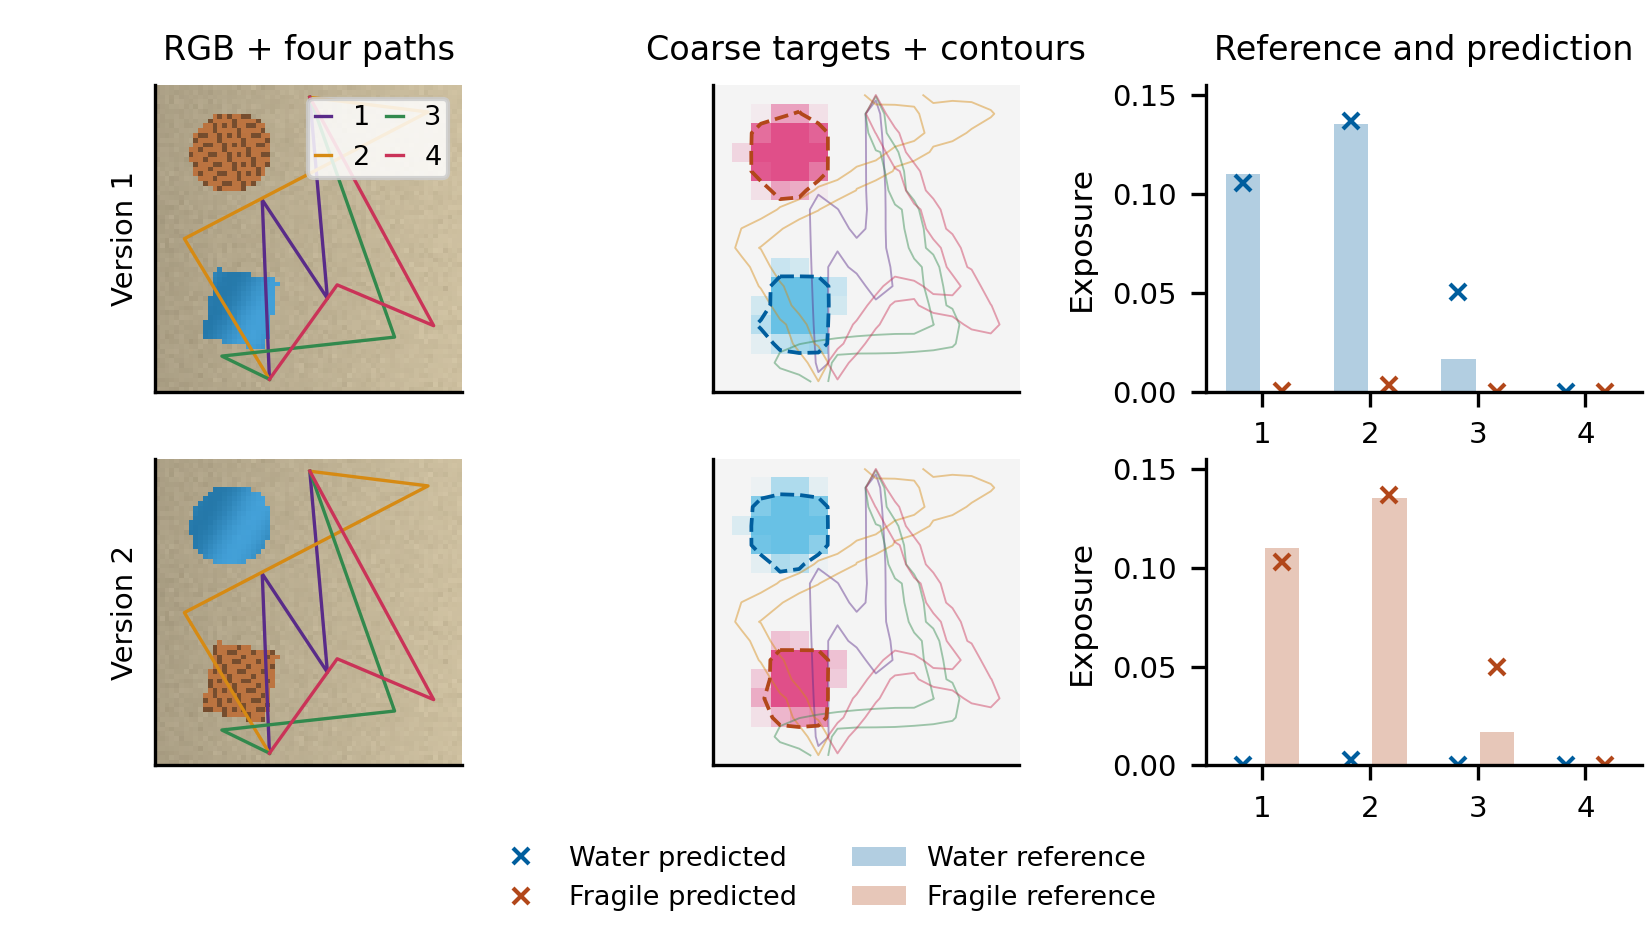
\includegraphics[width=\linewidth]{figures/task_scene.png}
\caption{Fixed first discovery scene and its exchanged-attribute version.
Left: RGB and candidate centerlines. Middle: source 64-to 16 targets (cyan: water;
magenta: fragile), footprint contours, and dashed predicted .5 contours. Right:
direct 512 and stored predicted exposures for all four candidates. Model seed 0
and scene index 0 were fixed independently of results. The display is
illustrative, not an estimate of event frequency.}
\label{fig:task}
\end{figure}

\paragraph{Learning setup.}
The predictor is a randomly initialized ResNet-18~\citep{resnet} with four lateral 1$\times $1
projections to 64 channels, bilinear top-down fusion, 3$\times $3 refinement, and
a two-channel output at 16$\times $16. Sigmoid outputs fit area-pooled binary
attribute masks using binary cross entropy plus soft Dice loss. Each fixed model
uses 800 training images, one version per scene, 24 epochs, batch size 20, and
960 AdamW updates (learning rate .001; weight decay .0001), with the final
checkpoint rather than validation-based selection. Color/polarity/contrast
augmentation preserves geometry. There are no high-resolution action-cost labels
or candidate-conditioned inputs to this training. We retain all five previously
fixed independent-geometry/source 64 checkpoints.

\paragraph{Public cost and actual deployment unit.}
Mean footprint exposures are $ e=(e_w,e_f)$. Cards A, C, and D define
\begin{equation}
g_A(e)=e_w,\qquad g_C(e)=e_w+e_f-e_we_f,\qquad g_D(e)=e_f.
\label{eq:cost}
\end{equation}
The trivial zero-cost card B is excluded from deployment. Each independent scene
draws one of the two image versions and one A/C/D card uniformly. The selector
minimizes predicted cost; ties within $10^{-9}$ use a stored independent uniform
draw. It chooses once, then accepts iff the estimate is at most $\tau=.02$.
Rejection never triggers reselection. The direct 512 attribute--footprint integral
and Eq.~\ref{eq:cost} define reference cost. It is a synthetic mean-exposure
criterion, not collision probability, traction, or execution success.

For acceptance $A$, reference cost $ c_\pi $ of the chosen action, and availability
$O=\ind\{\min_a c_{\mathrm{ref},a}\leq\tau\}$, report
\begin{equation}
C=\Prb(A),\quad R=\frac{\Prb(A,c_\pi>\tau)}{\Prb(A)},\quad
\eta=\frac{\Prb(A,c_\pi\leq\tau)}{\Prb(O=1)}.
\label{eq:metrics}
\end{equation}
$R$ is undefined for zero acceptance. The opportunity denominator contains only
the supplied four candidates; unsafe accepts never increase $\eta $. Scene-level
safe loss is $\Prb(O=1)-\Prb(A,c_\pi\leq\tau)$. A 2.70 percentage-point loss
over all scenes is different from a 3.39\% loss of available safe opportunities.

\section{What the uniform-cell interpretation changes}
\label{sec:mechanism}
Partition the fine grid into coarse cells $B$ with area weights $ w_B$. For one
binary property $P$ and footprint $F$, let $ p_B=\overline P_B$ and
$ f_B=\overline F_B$, and let $D=\sum_B w_B f_B>0$. The direct and separately
pooled exposures are
\begin{equation}
e_{\rm ref}=\frac{\sum_Bw_B\overline{PF}_B}{D},\qquad
e_{\rm pool}=\frac{\sum_Bw_Bp_Bf_B}{D}.
\end{equation}
Subtracting gives the elementary identity
\begin{equation}
e_{\rm pool}-e_{\rm ref}
=-\frac{\sum_Bw_B\operatorname{Cov}_B(P,F)}{D}.
\label{eq:covariance}
\end{equation}
This covariance describes spatial coincidence within a cell, not correlations
between training scenes. A half-occupied property and half-occupied footprint
give exposure .5 from their means, whether their true overlap gives exposure
zero or one. That example illustrates the operator; it is neither an empirical
frequency estimate nor an impossibility proof for our restricted shape family.

\paragraph{Uniform lifting clarifies the information claim.}
Let $\Pi $ replace a field by its mean in every coarse cell. Since $\Pi P$ is
constant there,
\begin{equation}
\int (\Pi P)(\Pi F)=\int (\Pi P)F.
\label{eq:lift}
\end{equation}
Thus separate pooling is equivalent to uniform lifting of the coarse property
followed by integration over the original footprint. A more detailed footprint
or constant upsampling alone cannot repair the measurement. An alternative
decoder could still use neighboring fractions to infer within-cell geometry.
The established claim is therefore residual decision error of the \emph{current
target--aggregation interface}, not an irreducible lower bound for every method
that reads coarse attributes.

\paragraph{Four levels under one footprint.}
We compare direct 512 exposure, separately pooled 512 exposure, the actual
source 64-to 16 target, and the learned field, always with the same F512 or its
exact nonoverlapping 32$\times $32 block means. For a fixed candidate,
\begin{align}
\widehat e-e_{\rm ref}
={}&(\widehat e-e_{\rm target 64})
 +(e_{\rm target 64}-e_{\rm pool 512})
 +(e_{\rm pool 512}-e_{\rm ref}).
\label{eq:telescope}
\end{align}
These terms isolate supervision-fit error, source-raster difference, and
aggregation error. We reapply Eq.~\ref{eq:cost} at every level before telescoping
\emph{cost} differences. In particular, summing the two channel exposure errors
does not give the nonlinear C cost error. Terms may oppose one another; their
absolute magnitudes cannot be interpreted as additive shares of final error.

We distinguish two analyses. \emph{Fixed selection} evaluates all levels at the
original model-selected action, isolating measurement changes from action
changes. \emph{Each-level reselection} lets each level choose once and accept,
then evaluates the selected action against the same direct reference. The latter
measures full decision consequences, including new failures outside the cases
that the uniform oracle originally lost.

\paragraph{Operating conditions and numerical scope.}
The covariance is zero when either binary field is constant within every cell.
For fractional occupancies, Cauchy--Schwarz yields the per-channel envelope
$D^{-1}\sum_Bw_B\sqrt{p_B(1-p_B)f_B(1-f_B)}$; the sum of channel envelopes also
bounds C's cost change because its partial derivatives lie in $[0,1]$.
We use joint fractional occupancy and pooled cost margin $|\poolcost-\tau|\leq .005$
as fixed diagnostic conditions. The envelope is an algebraic sensitivity bound,
not a new deployable safety algorithm. Near-threshold fragility itself is not
novel; the empirical question is its frequency and size in the stated generator.

Our precision check rasterizes properties at 1024, averages them to 512, and keeps
F512 fixed. It isolates property-raster sensitivity; it is not an exact continuum
or footprint-accuracy guarantee. Earlier full 256/direct 512 comparisons are
retained separately and are not attribution arms.

\section{Decision effects and one prospective confirmation}
\label{sec:evidence}
\paragraph{Consumed discovery.}
We use the already consumed E3 IID and new-appearance banks, 2,000 scenes each,
and all five fixed independent/source 64 models. Original image versions, cards,
ties, and stored predictions are retained. The analysis does not recertify any
rule. At fixed restored-model actions, pooled 512 versus direct 512 changes 3.68\%
of labels on IID and 3.83\% on new appearance, all reference-safe to pool-danger
in these observations. Descriptive crossed model/scene 95\% intervals are
[2.89\%,4.53\%] and [3.03\%,4.70\%]. The five models share 2,000 scenes; their
10,000 model--scene entries are not independent trials.

With independent selection by each oracle, pooled 512 loses 72/2,000 IID safe
opportunities (3.60 pp) and 77/2,000 appearance opportunities (3.85 pp). The actual
target 64 oracle loses 60 and 67 respectively. These are full-scene consequences,
not only differences on unselected high-cost candidates. The fixed-footprint
precision check changes .05\% of fixed-action labels on IID and none on appearance.
Pooling flips stable to that check remain 3.63\% and 3.83\%.

Signed cost terms at fixed IID selections are+.001807 from pooling, $-.000653$
from the source raster, and $-.000292$ from the model. On appearance they are
$.002060$, $-.000714$, and $-.001453$, giving total mean $-.000108$ despite mean
absolute error .003102. Model and net measurement terms oppose one another in
31.52\% and 32.49\% of decisions. These are signed cancellations, not causal
percentages attributed by summing absolute components.

\paragraph{Frozen prediction.}
This substantive signal motivates one new normal-IID bank of 2,000 scenes, with
unchanged models, generator, footprints, formulas, threshold, and ties. No new
training is performed. Anonymous continuous patch and full-scene identities have
no exact overlap with the 10,200 E2/E3 records, including training and validation.
This is a same-generator confirmation, not cross-task transfer. The three
predictions require: (H1) stable-reference lost-opportunity probability above .01
for pooled 512; (H2) conservative direction proportion above .90; and (H3) a
small-minus-larger margin flip-rate difference above .10 under joint boundary
overlap. Each claim has one-sided error budget $\gamma=.05/3$.

H1 uses an exact binomial lower bound. H3 uses an approximate crossed model/scene
bootstrap with only five model seeds. An additional stricter H2 scene-level
check was recorded after job submission but before inspecting any new outcome:
among scenes with any selected-action pooling flip across the five fixed models,
all flips in a scene must be conservative. It avoids a degenerate bootstrap lower
limit of one when every observed flip has the same direction. The original
protocol and output remain unchanged; Appendix~\ref{app:direction} gives the
timing and distinguishes the two estimands.

\begin{table}[t]
\centering\small
\caption{Prospective normal-IID confirmation. H1 is the original primary stable
pooled 512 endpoint; the target 64 result is supplementary to the full decomposition.
One-sided lower bounds use $\gamma=.05/3$; H3's bootstrap is approximate.}
\label{tab:confirmation}
\begin{tabular}{p{.39\linewidth}rrr}
\toprule
Prediction & Observation & Lower bound & Criterion\\
\midrule
H1: stable lost opportunities &61/2,000&2.29\%&$>1\%$\\
H2: only conservative changes in a changed scene &68/68&94.16\%&$>90\%$\\
H3: small-minus-larger margin enrichment &37.31 pp&26.06 pp&$>10$ pp\\
\bottomrule
\end{tabular}
\end{table}

\paragraph{What changes in decisions.}
The direct oracle has 1,592 safe opportunities. Pooled 512 accepts 1,529 with no
unsafe outcome observed, losing 63 opportunities (3.15 pp of all scenes). The
finer-property check also retains a safe candidate in 61 of those scenes: H1's
exact lower is 2.2869\%. The actual target 64 oracle accepts 1,540, of which two
are unsafe, so it loses 54/2,000 safe opportunities. This is 2.70 pp of all scenes
and 3.39\% of the 1,592 available opportunities. It is not a 2.7\% increase in
danger, nor a replacement of H1 after seeing results.

At the five models' fixed actions, pooling changes 322/10,000 labels (3.22\%,
descriptive 95\% interval [2.47\%,4.02\%]), all conservatively. Of these, 312 remain
when the finer-property check agrees with the reference label. The check itself
changes 15 labels (.15\%). Across all nontrivial candidate entries, its p 95 cost
difference is .000509, passing the fixed numerical screen. No observed zero-risk
count constitutes a new safety certificate.

\begin{figure}[t]
\centering
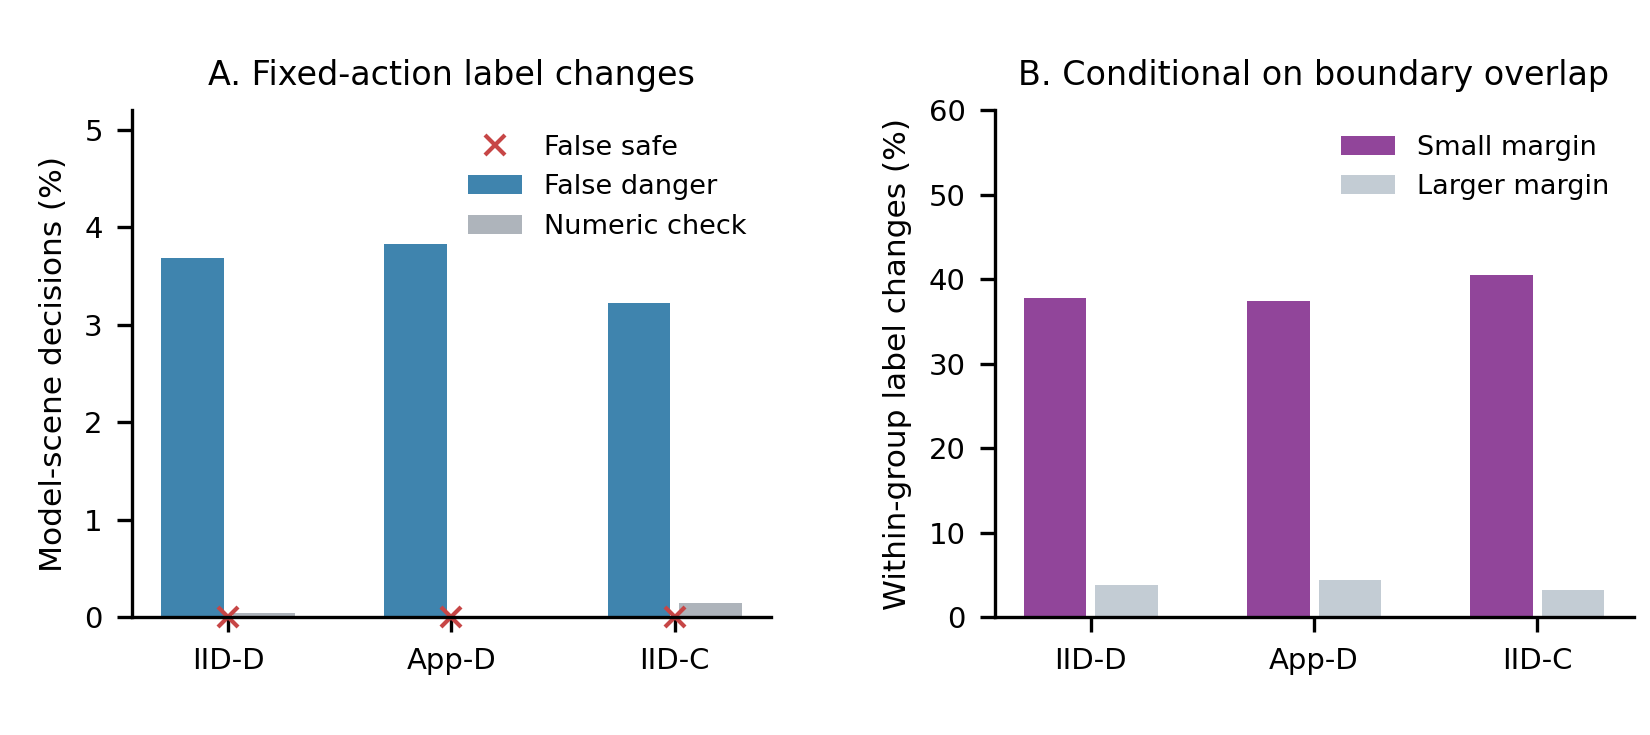
\includegraphics[width=\linewidth]{figures/oracle_confirmation.png}
\caption{Fixed-action label changes and their operating conditions. IID-D and
App-D are consumed discovery banks; IID-C is the prospective IID bank. A:
false danger means reference-safe to pooled-danger; false safe is the reverse
(no such flips observed). The numeric check holds the footprint fixed. B:
rates within overlapping-boundary groups, using the frozen .005 margin.
These are observed proportions; Table~\ref{tab:confirmation} supplies the
separate one-sided hypothesis comparisons.}
\label{fig:confirmation}
\end{figure}

Among overlapping-boundary actions, the frozen small-margin group has 40.57\%
label changes versus 3.26\% at larger margins. All 68 scenes with any flip across
models have only conservative flips, with exact conditional lower 94.1566\% for
the fixed model bank. The evidence confirms the predicted operating conditions
in the normal distribution. It does not make near-threshold sensitivity a new
general phenomenon, prove all pooling errors are positive, or establish that
every coarse decoder must lose these opportunities.

\section{One same-information reconstruction control}
\label{sec:comparison}
The preceding replacement fixes learning error but retains the aggregator.
We now test whether a different interpretation can exploit information already
present in neighboring coarse values. Development uses the consumed 2,000-scene
IID discovery bank. One implementation and two scalar offsets are fixed before
evaluating the already consumed 2,000-scene confirmation bank. This is an
\emph{appended baseline analysis}, not a new untouched confirmation. There is
no new training, dataset, resolution search, or risk certification.

\paragraph{Three treatments with identical action access.}
The primary track uses the perfect actual target 64 field; the secondary track
uses all five existing restored model fields. Uniform interpretation computes
the original exposure. All three treatments may access exactly the same F512,
so PLIC is not given better action geometry. The global shift subtracts one
constant after Eq.~\ref{eq:cost}. Its argmin is the original uniform argmin,
since translation preserves ranking; no clipping-induced ties are introduced.
From a fixed 13-value offset bank, development maximizes safe-accepted count
subject to no increase in observed unsafe-accepted count relative to uniform.
Ties favor the smallest absolute offset. The selected offset is .001 for the
target track and zero shared across the five learned models.

The only spatial alternative is the established Parker--Youngs PLIC construction
\citep{pilliod2004}. A fixed weighted 3$\times $3 gradient with center weight 2
estimates a cell's outward normal. A straight half-plane then matches the cell's
original fraction by analytic square-area inversion. Empty/full cells remain
unchanged; cells with gradient L1 norm at most $10^{-12}$ retain uniform occupancy
rather than an invented orientation. Exact line-cut fractions of fine pixel
squares are integrated against F512. Coarse predictions are neither thresholded
nor denoised. The reconstruction routine accepts only the coarse field and
footprints, never true patch parameters, fine property masks, reference costs,
or oracle boundary normals. It is a first-order PLIC baseline, not the
second-order ELVIRA method or a newly proposed algorithm.

\paragraph{Full-scene gains and harms.}
Table~\ref{tab:appended} reports every scene, including no-safe-candidate cases,
and both recovered and newly harmed decisions. PLIC recovers 44 of the target
oracle's 54 lost opportunities without newly losing a previously accepted safe
one. However, it introduces 16 unsafe accepts: total unsafe count rises from 2
to 18. Safe opportunity efficiency rises from 96.61\% to 99.37\%, while empirical
unsafe frequency among accepted rises from .13\% to 1.13\%. The frozen shift
recovers six opportunities and introduces three unsafe accepts.

\begin{table}[t]
\centering\small
\caption{Appended full-scene comparison relative to uniform interpretation.
Target counts use 2,000 scenes. Learned counts aggregate five models sharing
those scenes and are not 10,000 independent trials. ``New unsafe'' counts newly
unsafe accepted decisions; no previously unsafe accepts are resolved on this bank.}
\label{tab:appended}
\begin{tabular}{llrrrrr}
\toprule
Input & Interpretation & Recovered & New safe loss & New unsafe & $R$ & $\eta $\\
\midrule
Target 64 & Uniform &0&0&0&.13\%&96.61\%\\
 & Global shift &6&0&3&.32\%&96.98\%\\
 & PLIC &44&0&16&1.13\%&99.37\%\\
\midrule
Five models & Uniform &0&0&0&1.03\%&96.77\%\\
 & Global shift &0&0&0&1.03\%&96.77\%\\
 & PLIC &83&0&43&1.56\%&97.81\%\\
\bottomrule
\end{tabular}
\end{table}

The learned track also has a mixed outcome. PLIC recovers 83 safe model--scene
decisions and adds 43 unsafe accepts, with no new safe loss observed. Net safe
acceptance increases .83 pp (descriptive crossed 95\% interval [.51,1.19] pp), while
new unsafe acceptance increases .43 pp ([.20,.69] pp). The target track's net safe
gain is 2.20 pp ([1.60,2.85] pp). The selected learned shift is zero and changes no
outcome. Fixed-selection analysis yields the same recovery and new-unsafe totals
on this appended bank, so those totals are not explained solely by permission
to reselect; the event archive retains action identities and individual changes.

\begin{figure}[t]
\centering
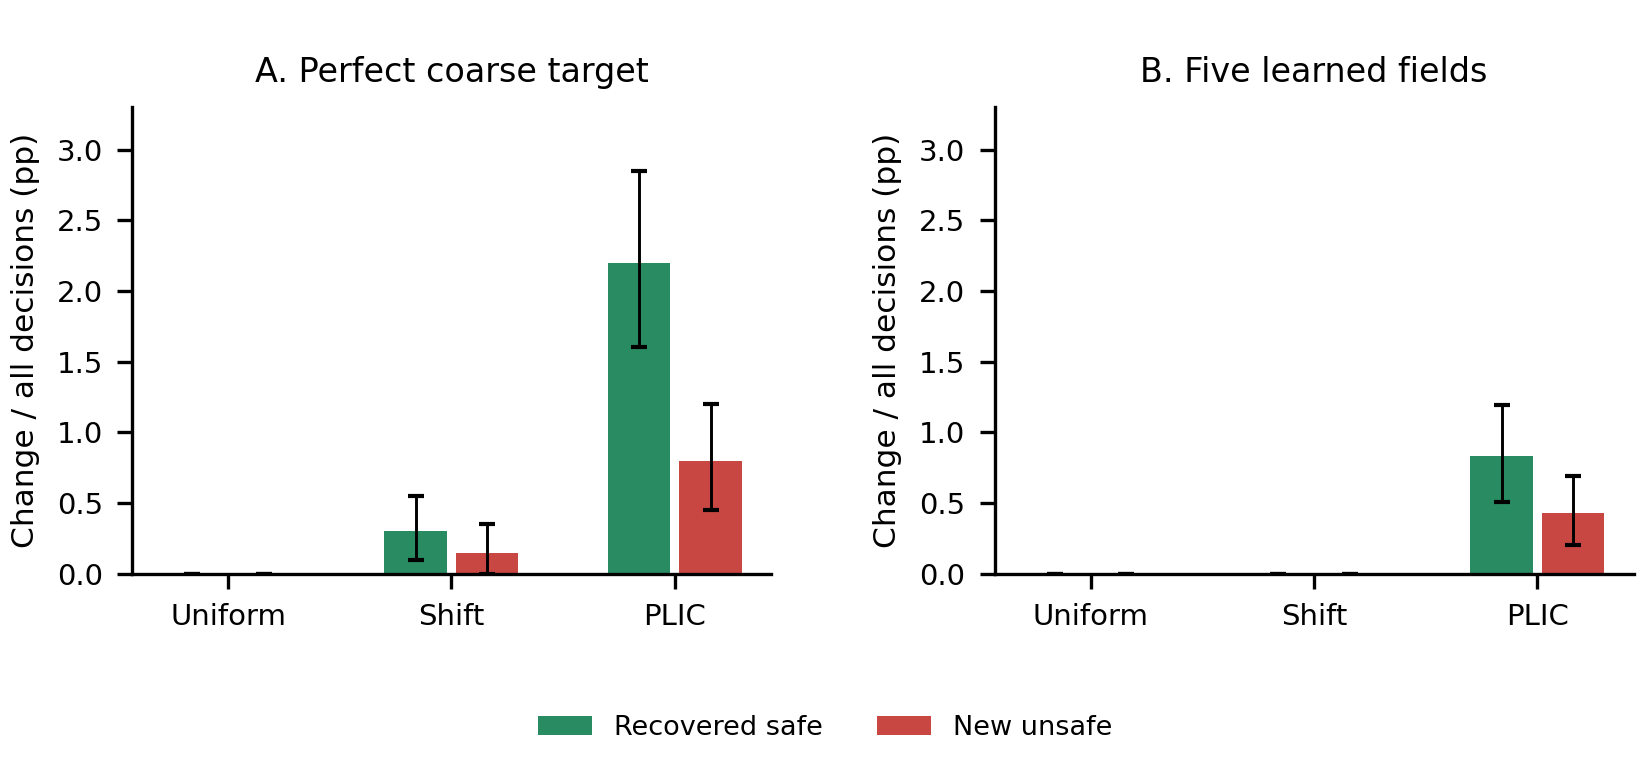
\includegraphics[width=\linewidth]{figures/same_information_tradeoff.png}
\caption{Opportunity recovery and newly unsafe acceptance must be read together.
PLIC uses the same coarse field and action information as uniform integration.
No new safe losses were observed, but both input tracks add unsafe accepts.
The offset was fitted under a development unsafe-count constraint that was not
imposed on PLIC; these selected points are not a matched-risk comparison.}
\label{fig:appended}
\end{figure}

\paragraph{A concrete cancellation failure.}
For 25 of the 43 newly unsafe learned decisions, the action stays unchanged,
baseline model and target-measurement errors have opposite signs, target-measurement
absolute error decreases under PLIC, and total absolute error increases. These
conditions are checked on each event, not inferred from aggregate means. For
the first such event in scene/model order, Table~\ref{tab:cancellation} shows
that both component absolute cost errors improve, yet their earlier
opposition disappears and the total underestimation worsens. All 43 events,
including the 18 not meeting this joint pattern, are retained. The example
supports a particular failure mechanism, not a claim that cancellation explains
every harmful change.

\begin{table}[t]
\centering\small
\caption{First event satisfying the stated cancellation pattern, in scene/model order. The same reference-unsafe action is rejected before reconstruction and accepted after it ($\tau=.02$). This is a conditional illustration; all 43 newly unsafe learned events remain in the archive.}
\label{tab:cancellation}
\begin{tabular}{lrr}
\toprule
Quantity on the same action & Uniform & PLIC\\
\midrule
Reference cost & +0.024972 & +0.024972\\
Target estimate & +0.031961 & +0.021431\\
Learned estimate & +0.021279 & +0.016964\\
Target-measurement cost error & +0.006989 & -0.003541\\
Model-relative-to-target cost error & -0.010682 & -0.004467\\
Total cost error & -0.003693 & -0.008008\\
Decision & Reject & Accept (unsafe)\\
\bottomrule
\end{tabular}
\end{table}


\paragraph{What this comparison establishes.}
The recovery demonstrates that the current coarse field contains spatial
structure usable by another interpretation; the original residual loss cannot
simply be called irreducible representation error. It does not demonstrate a
risk-free repair or universal superiority over scalar calibration. The chosen
offset is constrained not to add development unsafe outcomes, whereas PLIC is
not. The full development shift curve is therefore disclosed in
Appendix~\ref{app:shift}: larger offsets recover more opportunities at higher
risk. We do not tune another offset on the appended bank. The conclusion is to
separate supervision fidelity, spatial interpretation, and acceptance calibration,
and to re-evaluate the latter after changing the former. No earlier certificate
is inherited by either modified rule.

\section{Supporting controls and relation to earlier work}
\label{sec:discussion}
\paragraph{Learning and decision-rule effects remain distinct.}
A prior matched geometry $\times $ source-raster experiment trained 20 models at
equal budgets. Independent geometry improves new-appearance regret relative to
the balanced-anchor scheme at both source 48 and source 64, with crossed 95\%
intervals [.003101,.006853] and[.002850,.017690], each exceeding the predeclared
.001 effect threshold. This controls a genuine learning-related effect while
keeping common-reference scoring fixed. The intervention changes shape, size,
rotation, and position jointly; it does not isolate position alone.

Earlier fixed-weight and risk-control results are summarized in
Table~\ref{tab:support}; details are in Appendix~\ref{app:earlier}. They support
the argument without defining its novelty. E1 uses historical checkpoints and
consumed diagnostic data. E3 uses the five E2 independent/source 64 models with
1,600 new calibration and 2,000 test scenes per domain. Their residual and
certification results must not be treated as one within-model factorial test.

\begin{table}[t]
\centering\small
\caption{Supporting results from distinct earlier banks. E3's fixed-restored
rule was already certified in its original finite bank. Those certificates do
not transfer to the appended shift or PLIC rules. $R$ is unsafe among accepted.}
\label{tab:support}
\begin{tabular}{llrrr}
\toprule
Study/bank & Rule & Acceptance & $R$ & $\eta $\\
\midrule
E1 appearance & Inherited $-2$ &85.03\%&4.70\%&99.63\%\\
E1 appearance & Same weights, restored &80.97\%&1.73\%&97.83\%\\
E3 IID & Restored, fixed .02 &78.58\%&1.07\%&96.93\%\\
E3 IID & Selected certified threshold &81.29\%&2.51\%&98.82\%\\
E3 IID & Joint residual protection &0\%&Undefined&0\%\\
\bottomrule
\end{tabular}
\end{table}

Joint protection and selective-risk control protect different objects. If
nonnegative estimates have a joint residual quantile $ q>\tau $, adding that bound
necessarily rejects all actions. A rule controlling risk among accepted actions
need not protect every unselected candidate. The E3 exact-binomial finite-bank
procedure applies established Learn then Test principles~\citep{ltt}; its
success shows that an imperfect pipeline can be useful under a specified rule
and distribution. It neither validates its measurement interface nor supplies
certificates for modified aggregation.

\paragraph{Spatial reconstruction and task-specific representations.}
Volume-of-fluid reconstruction estimates an interface from grid-cell fractions.
\citet{pilliod2004} compare first- and second-order methods, including the
Parker--Youngs gradient reconstruction used here. That literature supplies both
a baseline and the reason not to equate uniform-cell failure with representation
impossibility. Our task has noisy learned fractions, swept action queries and
thresholded decisions, rather than interface advection; we do not introduce a
new reconstruction scheme or claim second-order accuracy for this baseline.

Lambda-Field studies the compatibility of occupancy representations and path-risk
integration~\citep{lambda2019}. Its collision-risk construction differs from our
public mean-exposure cost, but representation-dependent path risk is established
prior work. Task-based quantization likewise studies limited representations
in terms of a downstream objective rather than signal recovery alone
\citep{shlezinger2019}. Smart Predict, then Optimize explicitly separates
prediction and decision losses~\citep{spo}. Our narrower contribution is a
same-reference empirical attribution with actual acceptance effects, prospective
operating-condition evidence, and a same-information alternative interpretation.

Egocentric Conformal Prediction already addresses conservatism from safety-
irrelevant prediction errors~\citep{egocentric}. Conformal Decision Theory
calibrates decision loss directly~\citep{cdt}. Neither decision relevance nor
moving beyond prediction-set calibration is a novelty claim here. We use these
distinctions to keep measurement validity and the object of a statistical
guarantee separate.

\section{Limitations and conclusion}
\label{sec:limitations}
The task is synthetic, uses a known cost law, and restricts actions to four
candidates. Numerical checks condition on a fixed footprint and do not prove
continuum accuracy. Oracle boundary features are privileged diagnostics. The
prospective confirmation concerns the original mechanism; the added reconstruction
and shift are retrospective comparisons on consumed data. Five model seeds limit
training-distribution inference. A single first-order PLIC baseline cannot
characterize every same-information decoder, and successful oracle-input repair
would not by itself establish safe learned-model deployment.

An attempted real-image extension using RELLIS-3D~\citep{rellis} stopped before
mechanism evaluation because the geometric reference lacked independent error
bounds. Its initial 24-frame screen and subsequent prerequisite stop are retained
in the appendix; the planned new 48-frame set was never instantiated. It supplies
neither supporting nor refuting evidence for cross-task transfer. The extension
remains closed; no VLM, RL or external experiment is added.

Accurately realizing a coarse supervision target does not, by itself, validate
the action measurement implemented by its current aggregation rule. In this
controlled task, common-reference oracle replacements isolate a primarily
conservative aggregation effect with material opportunity loss and predictable
operating conditions. Distinguishing spatial interpretation from the underlying
information avoids an unsupported impossibility claim. The appropriate technical
choice is determined by what is recovered and what new errors are introduced,
not by component fit or recovered failures alone.

\label{maintextend}
\clearpage
\typeout{FIRST-STATEMENTS-PAGE=\thepage}
\section*{AI use statement}
Generative AI tools assisted with research questions and hypotheses, experimental
design, procedural-data and analysis implementation, mathematical exposition,
interpretation, literature discovery, figures, and manuscript drafting and editing.
Numeric results were produced by executable analysis, not inferred from generated
prose. Independent computational checks are documented in the appendix. This is
a working draft: human authors must review the AI-assisted contributions and
finalize responsibility statements before submission; completed human review is
not asserted here.
\section*{Reproducibility statement}
The appendix specifies data provenance, numerical definitions, fixed training,
the retrospective status of the appended comparison, and verification procedures.
Source freezes, results, and earlier negative outcomes are preserved internally.
The present manuscript source contains no personal paths or development-repository
links; an anonymous code supplement must still be finalized before submission.
\bibliography{references}
\bibliographystyle{iclr2027_conference}
\clearpage
\appendix
\section{Data separation and inference units}
E2 crosses two geometry schemes, source rasters 48/64 and five paired seeds
(20 models), with 800 training and 100 validation scenes per condition. Training
follows Section~\ref{sec:task}; the source rasters share RGB and the final
checkpoint is fixed without validation selection. Each independent-geometry
test bank has 400 scenes. Training uses one assignment version per scene;
evaluation retains both but samples one version/card for the actual decision.

E3 preselects all five independent/source 64 E2 checkpoints. It uses 400 development
scenes and, per domain, 1,600 calibration and 2,000 test scenes. The normal
generator and independent path sampler in Section~\ref{sec:task} operate before
rasterization; no pixel, risk or feasibility screen changes their sampling.

Oracle discovery reuses the consumed E3 IID/appearance test banks. The later
prospective bank has 2,000 new IID scenes (geometry seed 2612091301), with a recorded
source/checkpoint freeze before generation. Exact anonymous patch and complete-
scene identities are disjoint from all 10,200 E2/E3 records. IDs, appearance names,
seeds and path/patch ordering are excluded from the identity comparison; arbitrary
geometric symmetries are not quotient out. After that confirmation, the bank is
consumed. The PLIC/shift analysis in Section~\ref{sec:comparison} is explicitly
appended to it, without new samples or renewed confirmatory status.

Learned-track ratios pool five models over the same 2,000 scenes; crossed
bootstrap draws preserve that dependence. Target-oracle intervals resample
scenes only. Five training seeds still limit the approximate crossed inference.

\section{Spatial reference and reconstruction details}
The direct reference rasterizes each continuous property and swept-union footprint
at 512. It averages their product over footprint area, then applies the public
card law. It is a fixed discrete reference for synthetic mean exposure. The
auxiliary property check rasterizes properties at 1024, averages to 512 and retains
F512. An earlier full 256/direct 512 comparison changes both property and footprint
rasters and is kept separate from the common-footprint attribution.

\paragraph{Signed cost attribution.}
Exposure replacement follows Eq.~\ref{eq:telescope}. For every fixed action, cost
differences are separately evaluated as
\[
\widehat c-\refcost=(\widehat c-\targetcost)
 +(\targetcost-\poolcost)+(\poolcost-\refcost).
\]
The nonlinear formula is applied before differencing. Channel exposures,
signed/absolute costs and label-pattern transitions are preserved. The variance
envelope uses privileged reference occupancies; its zero-flip implications are
implementation checks.

\paragraph{PLIC area inversion.}
The normal is the negative weighted centered gradient of the coarse fraction,
with transverse weights $(1,2,1)$ and edge-replicated padding. Pairing differences
before summation eliminates roundoff-generated transverse components for an
exactly constant transverse field. Normalize $(n_x,n_y)$ by its L1 norm. For a
nonzero normal let $ a=|n_x|$, $ b=|n_y|$, $ a+b=1$, $ s=\min(a,b)$ and $ l=\max(a,b)$.
The area CDF of $ aU+bV$ for independent unit-square coordinates can be evaluated
symmetrically. At $0\le t\le 1/2$ its lower half is
\[
H(t)=\begin{cases}t^2/(2ab),&t<s,\\(t-s/2)/l,&t\ge s.\end{cases}
\]
Axis-aligned limits are handled analytically; the upper half uses $1-H(1-t)$.
For fraction $ p $, invert the lower tail $ q=\min(p,1-p)$ using
$ t=\sqrt{2abq}$ when $ q\le s/(2l)$, otherwise $ t=lq+s/2$; reflect for $ p>1/2$ and
translate for negative normal components. This yields a half-plane whose
unit-square area is the original $ p $.

For each fine pixel square, the same CDF gives its exact fractional area under
the reconstructed half-plane. Integrating those fractions against binary F512
preserves each coarse cell's original mass. Cells where a footprint is entirely
zero or one need no fine calculation: the integral is fixed by conserved mass.
All fractions, including small learned probabilities, are retained. A mixed
cell whose gradient L1 norm is at most $10^{-12}$ stays uniform. This is an
explicit fallback, not a inferred true boundary.

On the appended bank, the maximum analytic inverse-area discrepancy is
$2.78\times 10^{-16}$ and the maximum sum-of-fine-areas discrepancy is
$3.33\times 10^{-16}$, below the fixed $10^{-10}$ tolerance. There are 34,837
gradient-fallback cells across the input tracks and 5,047,140 reconstructed query
cells. These numerical checks establish conservation, not physical correctness
of the inferred boundary or a safety guarantee.

\section{Shift fitting and unequal risk points}
\label{app:shift}
The fixed cost-offset bank is
\[
\{- .02,- .015,- .01,- .005,- .002,- .001,0,.001,.002,.005,.01,.015,.02\}.
\]
One offset is fitted for perfect target input and one is shared across the five
model inputs. Fitting uses only consumed IID discovery data: maximize safe
acceptance subject to unsafe-accepted count no larger than uniform. Ties prefer
smallest absolute offset and then smaller offset. The rule is frozen at .001
for target input and 0 for learned input. It is empirical fitting, not a risk
certificate or guarantee that the same unsafe-count constraint will hold later.

The entire development bank is retained. At target offset .005, development has
1,578 safe and 17 unsafe accepts; at .01 it has 1,598 safe and 33 unsafe accepts.
Fixed PLIC has 1,600 safe and 16 unsafe accepts on development. The selected .001
shift has 1,550 safe and one unsafe accept. Larger shifts therefore can recover
more opportunities, and the selected point must not be interpreted as the
capacity of the whole shift family. No alternative offset is chosen using the
appended outcomes. The different risk levels preclude claiming a matched-risk
deployment advantage from the reported selected points.

\begin{table}[h]
\centering\small
\caption{Absolute appended outcomes. Learned rows pool five models sharing
2,000 scenes. The direct oracle has 1,592 safe opportunities per model.}
\begin{tabular}{llrrrr}
\toprule
Input & Interpretation & Accepted & Safe accepted & Unsafe accepted & Safe opportunities lost\\
\midrule
Target & Uniform &1540&1538&2&54\\
 & Shift &1549&1544&5&48\\
 & PLIC &1600&1582&18&10\\
Learned & Uniform &7783&7703&80&257\\
 & Shift &7783&7703&80&257\\
 & PLIC &7909&7786&123&174\\
\bottomrule
\end{tabular}
\end{table}

\section{Event-level cancellation evidence}
Each recovery, new safe loss, new unsafe accept and resolved unsafe accept keeps
its scene/model/card/action identity. At the original uniform-selected action,
write target-measurement error as $ m=c_{\rm target}-\refcost $ and model-relative
error as $ l=\widehat c-c_{\rm target}$. After changing interpretation, retain both
$ m'$ and $ l'$, with
$\widehat c'-\widehat c=(m'-m)+(l'-l)$. This fixed-action equality is checked
before interpreting reselected outcomes.

For the 43 newly unsafe learned PLIC decisions, 25 satisfy all of: unchanged
action, $ ml<0$ before modification, $|m'|<|m|$, and
$|m'+l'|>|m+l|$. The other 18 are retained as counterevidence to an exclusive
cancellation explanation. The first matching event in scene/model order is
scene 264, model index 1, exchanged version, card D, action 0. In it, both $|m|$
and $|l|$ decrease yet total underestimation grows, as detailed in the main text.
This is a transparent conditional illustration; it was not chosen to estimate
the population frequency of such cases.

\section{Prospective direction check and its addendum}
\label{app:direction}
The original confirmation uses one-sided budgets $.05/3$. H1 counts scenes where
direct 512 and the finer-property check both retain at least one safe candidate,
but pooled 512 fails to produce a safe accepted action. Its 61/2,000 events give
exact lower .02286937. H2 initially uses a crossed bootstrap for the fraction of
fixed-selected pooling flips that are conservative. Since all 322 flips are
conservative, its bootstrap lower degenerates to 1 and cannot establish population
certainty. H3 compares small/larger margin flip rates under joint boundary
overlap; its estimate is .373080 and approximate lower .260586.

The direction addendum was recorded at 20:57:54 UTC after job submission but
before any fresh outcome was inspected and before the original hypothesis file
was generated at 21:00:24 UTC. It is disclosed as a strengthening after the
original freeze, not silently included in that freeze. It requires an additional
exact scene-level check at the same H2 error budget: conditional on a scene
having any flip across the fixed five-model bank, every flip must be conservative.
All 68 changed scenes satisfy it; the exact lower is .941566. This conditional
fixed-bank estimand differs from the model--scene weighted proportion. Both
original outputs and the added check are preserved.

\section{Earlier controls and closed external attempt}
\label{app:earlier}
E1 uses five historical models and a consumed 300-scene calibration bank. With
restored output, positive-residual quantiles are .02797--.03287 for all 24
pair/version/card/candidate entries, .02201--.02767 for the current four
candidates, and .00501--.00790 for the fixed selected action. These are three
different protection objects. The smaller marginal selected-action bound does
not itself control unsafe frequency after acceptance.

E3 separately uses all five preselected E2 independent/source 64 models. Twelve
threshold rules per source/target calibration domain use exact one-sided
Clopper--Pearson upper bounds with family budget
$\delta/(5\cdot 2\cdot 12)=.05/120$. The desired conditional unsafe limit is
$\epsilon=.05$, distinct from danger threshold $\tau=.02$ and residual miscoverage
$\alpha=.05$. The original fixed .02 restored rules already certify, with source
upper bounds 1.66--2.54\%; selecting a higher-coverage certified threshold increases
both opportunity use and test risk. Source certificates do not become unknown-
distribution guarantees on appearance shift, and no old certificate applies to
PLIC or a newly fitted shift.

The RELLIS attempt evaluated a fixed 24-frame training-sequence pilot. All-four
corridor unknown area at most 5\% held in 0/24 cases; an optimistic diagnostic
discarding depth/occlusion checks reached 3/24. These results concern the chosen
single-scan surface-fit interface, not the dataset's general suitability. A
bounded revision inspected 240 raw scans around those same 24 development frames
and ran a motion-compensation prototype. Independent physical alignment and
visibility error bounds remained unresolved. It stopped before selecting,
acquiring or evaluating the planned new 48-frame set. This is a prerequisite
stop, not 0/48 and not a mechanism-transfer result; neither external training nor
an external final test was run.

\section{Computational verification}
The original oracle round has six distinct tests and independent replay of
52,000 discovery decisions and 26,000 prospective decisions, with 768 and 384
blockwise candidate-cost checks. The additional PLIC tests cover mass against
independent polygon clipping, uniform-lift identity, zero-gradient fallback,
complement/transposition behavior, axis orientation, and constant-footprint
cells. One initial test detected transverse roundoff at approximately
$8.3\times 10^{-16}$ for an exactly constant transverse field; changing the
arithmetic to pair differences before summing fixed it. The original test,
failed attempt, and unchanged scientific tolerance are retained; no development
scene was read before the repaired tests passed.

Independent appended verification replays 72,000 decisions and 65,536 fine-square
areas with polygon clipping. The maximum polygon difference is
$3.33\times10^{-16}$; the constant-lift identity differs by at most
$3.71\times10^{-14}$. It also verifies all 25 specified cancellation-pattern
events among the 43 new unsafe learned accepts. All computation runs on the cluster; frozen inputs and outputs are preserved.

\end{document}
